%TODO_MAR:  Status: Up for revision

\chapter{Weakly-coupled Carbon Spins}
Similar to how the electronic spin state can be controlled by adding and removing a term to the Hamiltonian we can also control the state of a Carbon--13 atom. The Hamiltonian of the nuclear spin depends on the electronic spin state\citep{Taminiau2014Universal}. A hyperfine term describing the interaction between the electronic spin and the nucleus is not present when the electron is in the $m_s = 0$ state :
 \begin{eqnarray}
H_0= \gamma_C B_z I_z \\
H_1 = \gamma_C B_z I_z +H_{\mathrm{HF}}
\end{eqnarray}

The hyperfine term consists of a contact term and a dipole term. For carbons with weak couplings \comment{TODO_MAR: Redefine weak coupling} (A$<$200kHz) the contact term is expected to be negligible and the dipole term is given by\cite{Lange2012Quantum}:

\begin{equation}
H_{\mathrm{dip}} = \frac{\mu_0 \gamma_e \gamma_C \hbar^2 }{4 \pi r^3} [ \bm{S \cdot I} - 3 (\bm S \cdot \hat{n_{\mathrm{hf}}})(\bm I \cdot \hat{n_{\mathrm{hf}}})]
\end{equation}

From this equation the parallel and orthogonal components of the Hyperfine interaction ($H_{\mathrm{dip}} = A_\parallel I_z + A_\perp I_x $), with respect to the NV axis along the z direction, can be derived to be:
 \begin{eqnarray}
A_\parallel= - \frac{\mu_0 \gamma_e \gamma_C \hbar^2 }{4 \pi r^3} \left(3\cdot \frac{z^2}{r^2}-1\right)\\
 A_\perp =  -\frac{\mu_0 \gamma_e \gamma_C \hbar^2 }{4 \pi r^3}\left( 3\cdot\frac{\sqrt{x^2+y^2}\cdot z}{r^2}\right)
\end{eqnarray}


\begin{figure}[htbp]
\centering
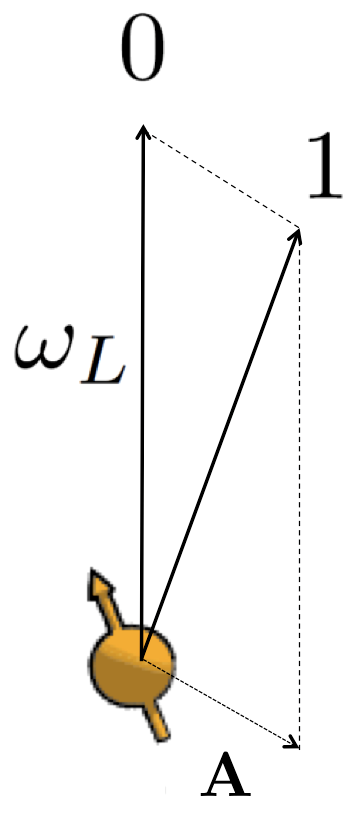
\includegraphics[keepaspectratio,width=0.2\textwidth,height=0.75\textheight]{./img/QuantizationAxis.png}
\caption{Flipping the electron spin from the  $m_s=0$ to the $m_s= +1$ state changes the quantization axis of $^{13}\mathrm{C}$ nuclear spins. For  $m_s=0$ spins precess about $\bm{\omega_L}$. For  $m_s=+1$ spins precess about a distinct axis $\bm{\tilde{\omega}}=\bm{\omega_L} +\bm{A}$.}
%removed reference to Tim's paper because it is already in the main text.
\label{fig:quantax}
\end{figure}




\section{Addressing weakly-coupled carbons trough dynamical decoupling}
\label{controllingacarbonthroughdynamicaldecoupling}
Spins precess about a quantization axis along $ \bm{\tilde{\omega}}$ with a frequency $|\bm{\tilde{\omega}}|$. We call $ \bm{\tilde{\omega}} $ the quantization-vector. When the electron is in the $m_s=0$ each nuclear spin precesses about $\bm{\tilde{\omega}} = \bm{\omega_L}$ with the Larmor frequency. The magnetic field is aligned along the quantization axis of the NV- center and defined as the z-direction.When the electron is in the $m_s=+1$ state nuclear spins precess about a distinct axis $\bm{\tilde{\omega}}=\bm{\omega_L} +\bm{A}$ \citep{Taminiau2012Detection}. The hyperfine interaction $\bm{A}$ depends on the position of that particular nuclear spin relative to the NV- center.

To understand how a Carbon--13 atom can be controlled it is useful to consider three situations. In the first situation the $\bm{\omega_L}$ and $\bm{A}$ point in the same direction. In the second situation $\bm{\omega_L}$ and $\bm{A_\perp}$ are of comparable magnitude, resulting in a large angle between the quantization axes. In the last situation $|\bm{A}|$ is small compared to  $\bm{|\omega_L|}$ resulting in a small angle between the quantization axes.

When applying a decoupling sequence with N\slash 2 decoupling units of the form {$\tau - \pi -2\tau-\pi-\tau$}, where $\tau$ is a wait time between pulses and $\pi$ is a $\pi$-pulse that flips the electron-state, the nuclear spin alternately rotates around the  $\bm\omega_L$ and the $\bm{\tilde{\omega}}$ axis. The net result of one such decoupling sequence is a rotation around an axis $\bm{\hat{\mathrm{n_i}}}$ by an angle $\phi$. Where $\bm{\hat{\mathrm{n_i}}}$ depends on the initial state of the electron: $\bm{\hat{\mathrm{n_0}}}$ when the electron starts in $m_s = 0$ and $\bm{\hat{\mathrm{n_1}}}$ when the electron starts in $m_s = +1$~\citep{Taminiau2012Detection}.

When $\bm{\omega_L}$ and $\bm{A}$ point in the same direction, the net rotation axis is independent of the initial electron-state making it impossible to use the electron to control the Carbon--13 atom using this decoupling sequence.

In the case where $\bm{\omega_L}$ and $\bm{A_\perp}$ are of comparable magnitude the net rotation axes $\bm{\hat{\mathrm{n_i}}}$ are strongly dependent on the initial electron-state for almost any $\tau$. Having one of these carbon atoms can make it hard to selectively control other carbons as there are very few inter-pulse-delays $2\tau$ for which only the carbon atom without the strong orthogonal-hyperfine is affected.

When considering the case where $\bm{|A|}$ is small compared to  $\bm{|\omega_L|}$ the net rotation axes  $\hat{n_0}$ and $\hat{n_1}$ are practically parallel and the nuclear spin undergoes an unconditional evolution. Only when the inter-pulse delay is precisely resonant with the spin dynamics the axes are anti-parallel leading to a conditional rotation\citep{Taminiau2012Detection}. The resonant condition occurs at:

 \begin{equation}
\tau = \frac{(2k+1)\pi}{2 \gamma_C B_z + A_\parallel}
\label{eq:res_dip_loc}
\end{equation}

And for $\omega_L \gg |\bm{A}|$ the dip has a width of:

 \begin{equation}
\Delta = \frac{A_\perp}{2\cdot (\gamma_C B_z)^2}
\label{eq:res_dip_width}
\end{equation}

If  $\hat{n_0}$ and $\hat{n_1}$ are not parallel, the resulting conditional rotation of the nuclear spin generally entangles the electron and nuclear spins. As a result, for an unpolarized nuclear spin state, the final electron spin state is a statistical mixture of $|x\rangle$ and $|-x\rangle$ when starting from the $|x\rangle$  state. Where the probability that the initial state is preserved is given by:

\begin{equation}
P_x = (M+1)/2
\end{equation}

With for a single nuclear spin:

\begin{equation}
M = 1-(1 - \hat{\bm{\mathrm{n_0}}} \cdot \hat{\bm{\mathrm{n_1}}}) \sin^2 \frac{N\phi}{2}
\end{equation}

\section{Characterizing the Nuclear-spin environment}

In reality the electron is not interacting with a single carbon but with a bath of carbon atoms. When the electron interacts with multiple carbons at the same time the contrast $M$ is given by the product of all individual values $M_j$ for each individual spin $j$. In order to selectively control one carbon the electron should not entangle with any other carbon when addressing it.
%Explain how fingerprint works and how it characterizes how many carbon we can control.
% IF selective, M goes all the way down. If a lot go to 0.5 as all coherence is lost.

To identify promising resonances for carbon control we perform a dynamical decoupling spectroscopy\citep{Taminiau2012Detection} or fingerprint. In a fingerprint experiment the electron is prepared in the $|X\rangle = |0\rangle +|1\rangle$ state. It is subjected to a decoupling sequence consisting of N/2 blocks of the form {$\tau - \pi -2\tau-\pi-\tau$}, and concluded by measuring $\langle X\rangle $. The fingerprint is the result of many repetitions for a range of inter-pulse delays $2\tau$. A narrow dip in the fingerprint spectrum is an indication a selectively controllable carbon.

By sweeping the number of $\pi$-pulses on such a dip it can be verified if it corresponds to a single carbon. If entanglement is created with a lot of spins at once all coherence is lost and contrast will go to 0. Only if no entanglement is created with any other carbon can the contrast be sweeped to -1. %This weird wording is used because it is possible that the response of another carbon is non existent exactly when the first one reaches -1. Maybe also add the in between case for few spins?

% NOTE: Extremely strongly coupled carbons are not in here
Because Carbon-13 atoms are randomly distributed in diamond there is a wide range of possible hyperfine strengths. In the ideal case the spectrum would be filled with well-separated narrow resonances. This would correspond to carbons lying mostly along the NV-axis, ensuring weak orthogonal-components of the hyperfine interaction, and a decreasing density of carbon-13 atoms the further one goes away from the NV-center. Although such a distribution would not occur naturally this ideal case can be useful in understanding fingerprints.
%ideal nicely seperated, narrow dips
% Interesting geometry springs to mind :) string of carbon-13 atoms in a grown diamond with increasing separation further from the diamond.

Most carbon-spins have very similar hyperfine-interaction strengths as they are relatively far away from the NV-center. This causes their resonances to overlap manifesting itself as a broad feature with little coherence in the fingerprint. We identify this response as the spin-bath.
% reality most far away -> similar strengths ->  spin bath response

Spins that have a strong hyperfine-interaction relative to other spins show up outside or at the edge of the spin-bath response. Going to higher orders $k$ separates resonances further allowing for control of more spins. As computations are fundamentally limited by the coherence time there is a limit to the resonance-order that can be used to address carbons. Additionally some of the relatively strong-coupled spins also have a strong orthogonal component of the hyperfine interaction. This orthogonal-component causes a broad response, effectively blocking a large range of $\tau$ from being used to control other spins.

% need the stronger
% sometimes one that is to strong -> increase B-field
Both these issues can be addressed by increasing the magnetic field. By increasing the magnetic field until the orthogonal hyperfine-components of all spins are small relative to the Larmor frequency the broad resonances that cause large parts of the spectrum to become useless disappear. Additionally all resonances move closer to $\tau =0$ while at the same time becoming narrower, allowing higher order resonances to be addressed within the coherence time.

% to much B-field -> to narrow dips, cannot address anymore (tech limitation)
Increasing the magnetic field will not always improve the situation. When the magnetic field is too strong the resonances become narrower than the resolution of the Arbitrary Waveform Generator used to generate the pulses that address the resonances, making it impossible to address these resonances effectively.
There are also practical limitations to how much the magnetic field can be increased. \citep{}
% Optimum B-field range 300-700

Similarly it is not practical to increase the magnetic field to compensate for arbitrary strongly coupled carbon-spins. \comment{WHY!?}
%sims indicate optimum B? of behouden voor appendix?
% Additional problems with B. Stability? -> appendix. transitions in excited states?





% Way to strong -> remove be pre-selecting samples


%Rand dist -> Range coupling sterktes
% als niet sterk orth -> parr -> mooie dip, te zwak -> veel vergelijkbare sterkte
% -> sommige sterk orthogonaal -> fucked
% Hogere ordes-> verder uit elkaar -> nadeel langere control times
% en B-veld -> zwakker otrhogonaal dus mooiere dips -> nadeel smaller -> te small -> optimum







% It also means that resonances of weakly coupled (with respect to the Larmor frequency) carbons must not overlap. This excludes those carbons that are very weakly coupled in absolute terms as resonances of these carbons are located closely together.

% As carbon--13 atoms are randomly distributed in the crystal the amount of weak resonances that can be addressed varies from NV to NV. By increasing the magnetic field the width and the delay-time of the resonances decreases. The downside is that it becomes harder to address these resonances as the resolution of the AWG used to apply the pulses is finite.

% TODO_MAR: Change ending of this chapter to bridge to next section better

% Section containing fingerprint measurements with identified Carbons and Ramsey measurements used to determine the coupling strengths.
% Also note that we have very strong orthogonal components
% T2 measurements ? Ramsey type experiments. Would require explaining what T2 is (or maybe not).

% Fingerprint graph with dips that are being addressed and fits of these resonances


% Table with T2*, HF_parr, HF_orth. Values can be found in QEC LT/Simulations/Hans_Sil01_Spin_Control
% B_field = 304.22G
\begin{figure}[htbp]
    \centering
    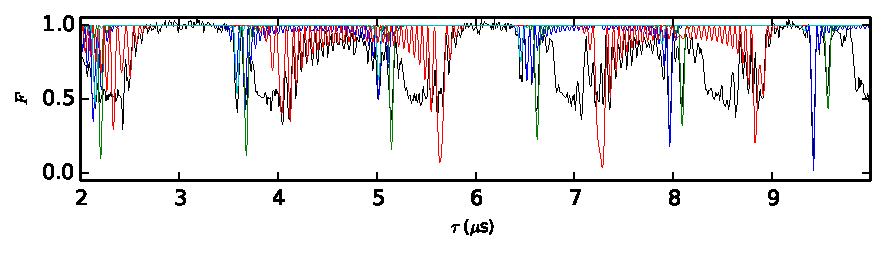
\includegraphics{Img/Truefingerprint.pdf}
    %TODO_MAR: use annotations to add labels in the graphs using matplotlib
    \caption{Fingerprint of Hans Sil01 at B = 304.12G for N=32 pulses.Larmor revival clearly visible. }
    \label{fig:FP}
\end{figure}

\begin{table}[htbp]
    \begin{tabular}{lllll}
    Carbon &  $A_{\parallel} $ & $A_{\perp}$ \\ \hline
    1         & 30.0 kHz$\cdot 2 \pi$             & 80.0 kHz$\cdot 2 \pi$                \\
    2         & 27.0 kHz$\cdot 2 \pi$             & 28.5 kHz$\cdot 2 \pi$              \\
    3         & -51.0 kHz$\cdot 2 \pi$          & 105.0 kHz$\cdot 2 \pi$              \\
    4         & 45.1 kHz$\cdot 2 \pi$           & 20.0 kHz$\cdot 2 \pi$                \\
    \end{tabular}
    \caption{Hyperfine paramters used to fit spins 1 to 4 in \autoref{fig:FP}.}
    \label{tbl:HF_par}
\end{table}

\begin{figure}[t]
    \begin{subfigure}[t]{0.49\textwidth}\centering
    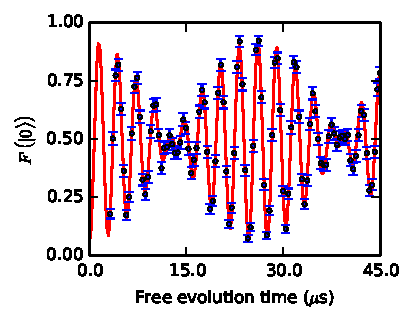
\includegraphics{Img/CarbonRamsey_C1.pdf}
    \caption{Nuclear Ramsey of Carbon 1} \label{fig:CR_C1}
    \end{subfigure}
    \begin{subfigure}[t]{0.49\textwidth}\centering
        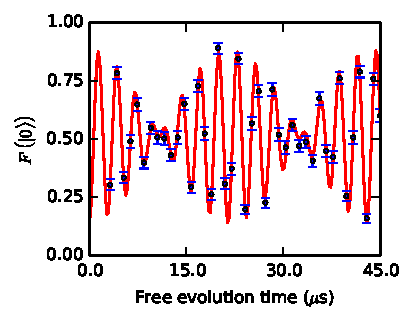
\includegraphics{Img/CarbonRamsey_C4.pdf}
        \caption{Nuclear Ramsey of Carbon 4}
        \label{fig:CR_C4}
    \end{subfigure}
    \caption{Nuclear Ramsey experiment wit}
\end{figure}



\section{Controlling weakly coupled carbons trough the electronic spin}
% Section containing theory (Gate circuits) on how to initialize and readout carbons





\section{Carbon Initialization \& Readout}
% TODO_MAR: Discuss naming of sec: Carbon Init&RO and Carbon Tomo
%  Section containing experimental results (Tomographies)
%  Should emphasize difficulty in seperating initialization and RO fidelity, what is not working? Is it working?




